\documentclass[tikz, border=12pt]{standalone}
\usepackage{tikz}
\usepackage{amsmath}
\usetikzlibrary{arrows.meta, positioning, backgrounds, fit}

\definecolor{simcolor}{RGB}{220,232,252}
\definecolor{simborder}{RGB}{70,100,180}
\definecolor{policycolor}{RGB}{255,213,170}
\definecolor{policyborder}{RGB}{210,70,40}
\definecolor{rewardcolor}{RGB}{255,243,210}
\definecolor{rewardborder}{RGB}{200,140,40}
\definecolor{ppocolor}{RGB}{240,228,255}
\definecolor{ppoborder}{RGB}{120,60,180}
\definecolor{currcolor}{RGB}{220,242,220}
\definecolor{currborder}{RGB}{50,140,50}
\definecolor{obscolor}{RGB}{214,229,252}
\definecolor{panelbg}{RGB}{250,250,250}

\begin{document}
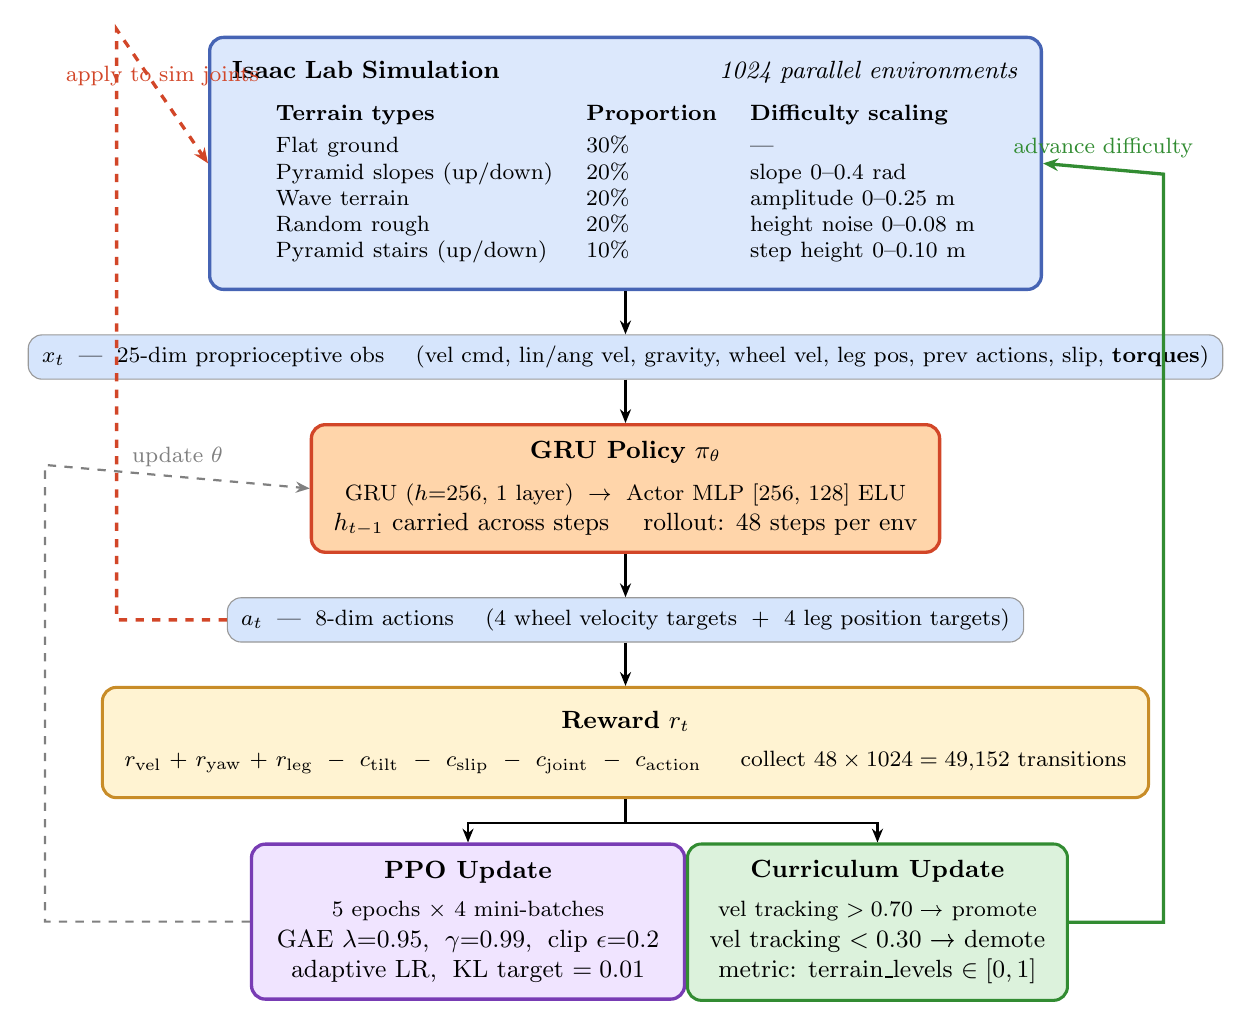
\begin{tikzpicture}[
    every node/.style={font=\small},
    box/.style={draw, rounded corners=5pt, align=center,
                inner xsep=8pt, inner ysep=6pt},
    simbox/.style={box, fill=simcolor, draw=simborder, line width=1.2pt},
    policybox/.style={box, fill=policycolor, draw=policyborder, line width=1.2pt},
    rewardbox/.style={box, fill=rewardcolor, draw=rewardborder, line width=1.1pt},
    ppobox/.style={box, fill=ppocolor, draw=ppoborder, line width=1.2pt},
    currbox/.style={box, fill=currcolor, draw=currborder, line width=1.1pt},
    smallbox/.style={box, fill=obscolor, draw=black!40, inner xsep=5pt, inner ysep=4pt},
    arr/.style={-{Stealth[length=5pt,width=4pt]}, thick},
    darr/.style={-{Stealth[length=5pt,width=4pt]}, thick, dashed, color=black!50},
    redarr/.style={-{Stealth[length=5.5pt,width=4.5pt]}, line width=1.2pt, color=policyborder, dashed},
    greenarr/.style={-{Stealth[length=5.5pt,width=4.5pt]}, line width=1.2pt, color=currborder},
]

%% ── Simulation Environment (top) ────────────────────────────────────────────
\node[simbox, minimum width=10.5cm, minimum height=3.2cm, text width=10.0cm]
  (sim) at (0, 0)
  {%
    \textbf{Isaac Lab Simulation} \hfill \textit{1024 parallel environments}\\[6pt]
    \footnotesize
    \begin{tabular}{lll}
      \textbf{Terrain types} & \textbf{Proportion} & \textbf{Difficulty scaling} \\[2pt]
      Flat ground            & 30\%  & — \\
      Pyramid slopes (up/down) & 20\% & slope $0$–$0.4$ rad \\
      Wave terrain           & 20\%  & amplitude $0$–$0.25$ m \\
      Random rough           & 20\%  & height noise $0$–$0.08$ m \\
      Pyramid stairs (up/down) & 10\% & step height $0$–$0.10$ m \\
    \end{tabular}
  };

%% ── Observation label ────────────────────────────────────────────────────────
\node[smallbox, below=0.55cm of sim]
  (obsnode)
  {\footnotesize $x_t$ \;—\; 25-dim proprioceptive obs \quad
   (vel cmd, lin/ang vel, gravity, wheel vel, leg pos, prev actions, slip, \textbf{torques})};

%% ── GRU Policy ───────────────────────────────────────────────────────────────
\node[policybox, minimum width=7.0cm, minimum height=1.5cm,
      below=0.55cm of obsnode]
  (policy)
  {\textbf{GRU Policy} $\pi_\theta$\\[4pt]
   \footnotesize
   GRU ($h{=}256$, 1 layer) \;$\rightarrow$\; Actor MLP [256, 128] ELU\\
   $h_{t-1}$ carried across steps \quad rollout: 48 steps per env};

%% ── Action label ─────────────────────────────────────────────────────────────
\node[smallbox, below=0.55cm of policy]
  (actnode)
  {\footnotesize $a_t$ \;—\; 8-dim actions \quad
   (4 wheel velocity targets \;$+$\; 4 leg position targets)};

%% ── Reward ───────────────────────────────────────────────────────────────────
\node[rewardbox, minimum width=10.5cm, minimum height=1.4cm,
      below=0.55cm of actnode]
  (reward)
  {\textbf{Reward} $r_t$\\[3pt]
   \footnotesize
   $r_\text{vel}$ + $r_\text{yaw}$ + $r_\text{leg}$
   \;$-$\; $c_\text{tilt}$ \;$-$\; $c_\text{slip}$
   \;$-$\; $c_\text{joint}$ \;$-$\; $c_\text{action}$
   \hspace{1em}
   collect $48 \times 1024 = 49{,}152$ transitions};

%% ── PPO Update ───────────────────────────────────────────────────────────────
\node[ppobox, minimum width=5.5cm, minimum height=1.4cm,
      below=0.55cm of reward, xshift=-2.0cm]
  (ppo)
  {\textbf{PPO Update}\\[3pt]
   \footnotesize
   5 epochs $\times$ 4 mini-batches\\
   GAE $\lambda{=}0.95$,\; $\gamma{=}0.99$,\; clip $\epsilon{=}0.2$\\
   adaptive LR,\; KL target $= 0.01$};

%% ── Curriculum ───────────────────────────────────────────────────────────────
\node[currbox, minimum width=3.8cm, minimum height=1.4cm,
      below=0.55cm of reward, xshift=3.2cm]
  (curr)
  {\textbf{Curriculum Update}\\[3pt]
   \footnotesize
   vel tracking $> 0.70$ → promote\\
   vel tracking $< 0.30$ → demote\\
   metric: terrain\_levels $\in [0,1]$};

%% ── Main vertical arrows ─────────────────────────────────────────────────────
\draw[arr] (sim.south)    -- (obsnode.north);
\draw[arr] (obsnode.south) -- (policy.north);
\draw[arr] (policy.south) -- (actnode.north);
\draw[arr] (actnode.south) -- (reward.north);
\draw[arr] (reward.south) -- ++(0,-0.3) -| (ppo.north);
\draw[arr] (reward.south) -- ++(0,-0.3) -| (curr.north);

%% ── Action feedback: policy output loops back to sim (left side) ─────────────
\draw[redarr]
  (actnode.west) -- ++(-1.4, 0)
  -- ++(0, 7.5)
  -- node[above, font=\footnotesize]{apply to sim joints} (sim.west);

%% ── PPO updates policy weights ───────────────────────────────────────────────
\draw[darr]
  (ppo.west) -- ++(-2.6, 0)
  -- ++(0, 5.8)
  -- node[above, font=\footnotesize]{update $\theta$} (policy.west);

%% ── Curriculum updates terrain difficulty ────────────────────────────────────
\draw[greenarr]
  (curr.east) -- ++(1.2, 0)
  -- ++(0, 9.5)
  -- node[above, font=\footnotesize]{advance difficulty} (sim.east);

\end{tikzpicture}
\end{document}
